\section{\aimOne}

\begin{frame}{\qOne}
	\textbf{Hypothesis:} deep learning spatial models will outperform point process models
	\begin{itemize}
		\item Extract neuron fluorescent traces $\rightarrow$ build RNN
		\item Raw fluorescent observations $\rightarrow$ convolutional deep learning model
		\item Compare prediction performance on withheld test data
	\end{itemize}
\end{frame}

\note{
	The main buy-in for this talk is that having an  accurate model of brain dynamics is useful. Most approaches today for brain-wide modeling use hand-crafted features in a  preprocessing pipeline that throws away spatial information. How much better can we do at predicting activity if we do not constrain our modeling by biological plausibility?
}

\begin{frame}{ 2P Experimental setup }
	\centering
	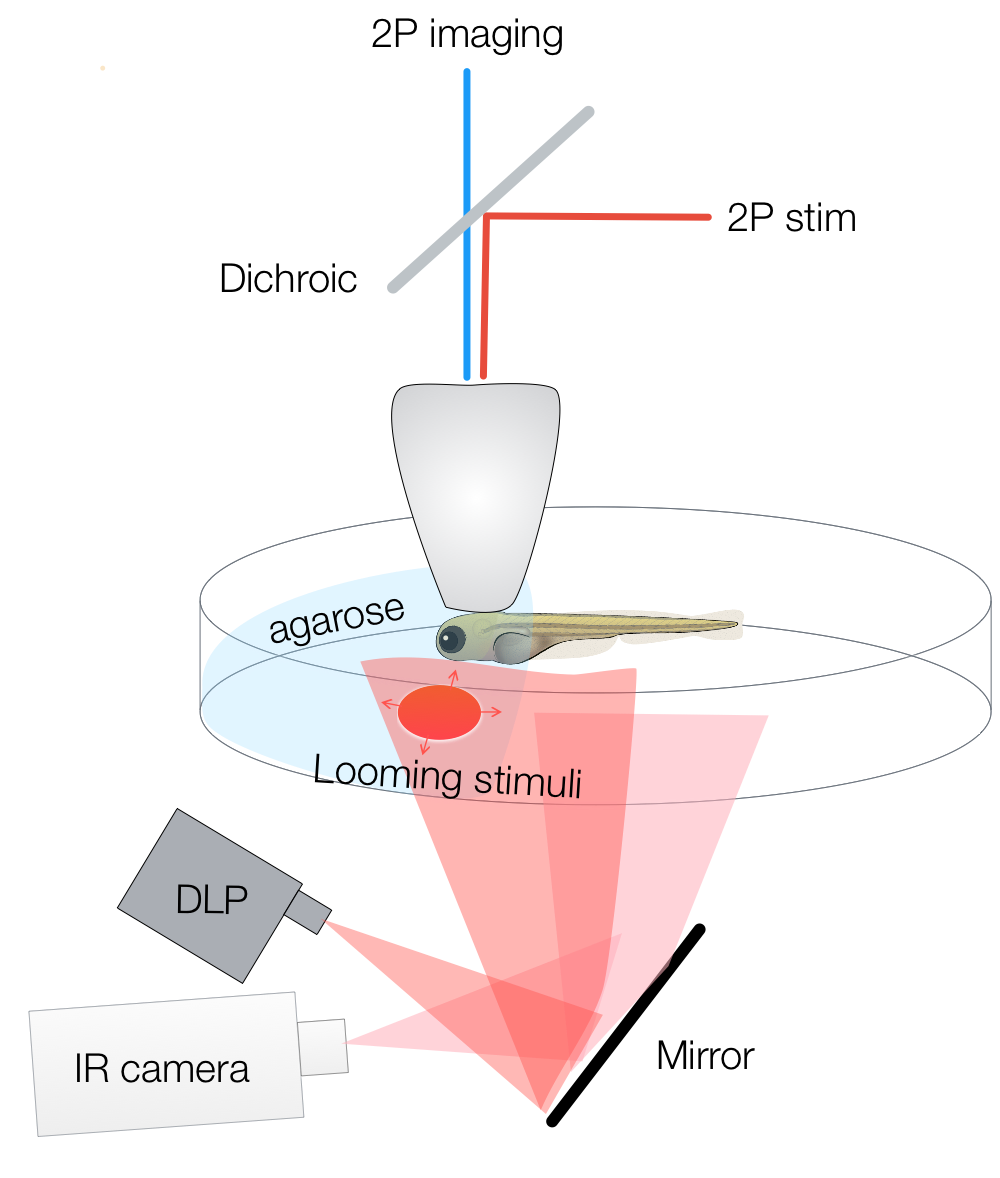
\includegraphics[height=\textheight]{media/experimental_setup.png}
\end{frame}{}

\begin{frame}{ Whole-brain 2P calcium imaging }{Z-projection of 19 planes, 4x real-time, 2Hz}
	% TODO make video shorter
	% center figure larger than textwidth
		\movie[]{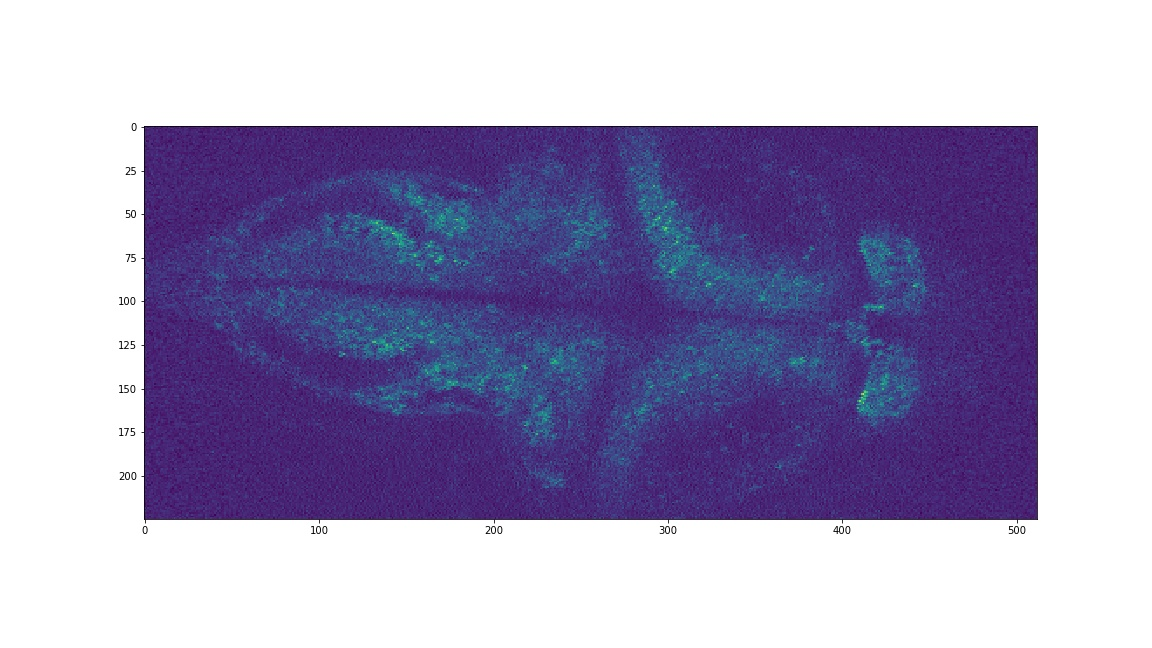
\includegraphics[width=0.6\textwidth,center]{media/20190429_f5e2.jpg}}{media/20190429_f5e2.mp4}
		\vspace{-20mm}
		\centering
		\begin{turn}{-90}
				\begin{minipage}{0.7\textheight}
					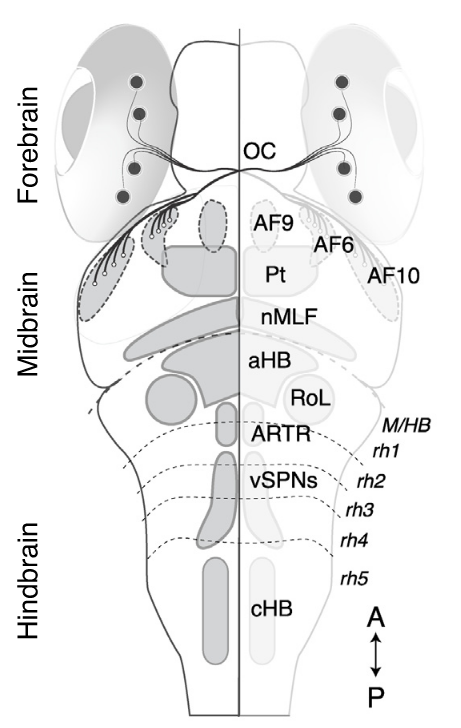
\includegraphics[height=0.5\textheight]{media/larval_atlas}
			 \end{minipage}
		 \end{turn}

	 % 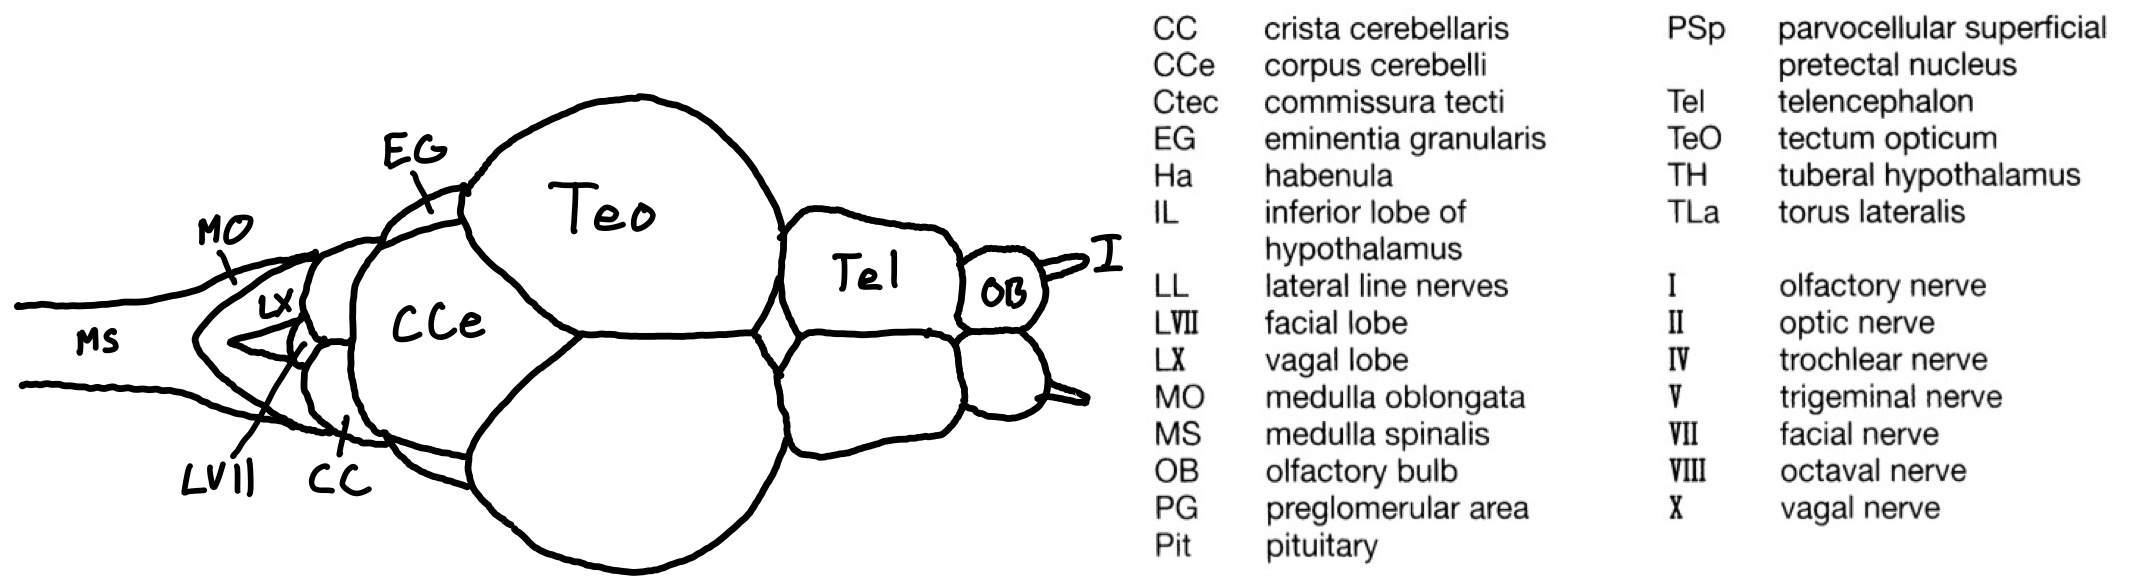
\includegraphics[height=0.5\textheight]{media/atlas}
	 \nakedfootnote{Naumann, Fitzgerald, et al. 2016}

	\note{need to change 2P offset for bidirectional imaging: ~2px jitter line-to-line}
	\note[item]{resting state video, no external stimuli}
	\note[item]{highlight brain deformation during tail movement}
	\note[item]{This is a video. About 2/3 way through, brain goes completely dark (!!), then whole brain lights up.}
\note[item]{Dorsal overview of zebrafish neuroanatomy. DSRGCs (black dots) project via the optic chiasm (OC) to ten contralateral retinal arborization fields(AFs). Pt,pretectum; nMLF, nucleus of the medial longitudinal fasciculus; aHB, anterior hindbrain; RoL, neurons in rhombomere 1; ARTR, anterior rhombencephalic turningregion; vSPNs, ventromedial spinal projection neurons; cHB, caudal hindbrain; M/HB, midbrain-hindbrain border; rh1–5, rhombomeres 1–5. A, anterior; P,posterior.}
\end{frame}


\begin{frame}{ Current approaches to brain-wide modeling }
	% \setcounter{footnote}{1}
	\begin{multicols}{2}
		\adjincludegraphics[width=0.6\textwidth,trim={0 {.42\height} 0 0},clip]{media/caiman.jpg}
		Extract neuron traces\nakedfootnote{Giovannucci et al. 2019.}
		\note<1>{In the early days of machine vision, researchers often used handcrafted feature extracters like edge detection to extract lower dimensional features that are then fed into a model. Today, neuroscience is similar: we motion correct a raw movie, identify independent spatial components, separate the sources, and attempt to whiten the signal based on assumptions of calcium indicator dynamics.}
		\vfill\null\columnbreak
		\uncover<2>{
			\adjincludegraphics[width=0.4\textwidth,trim={0 {.7\height} {.65\width} 0},clip]{media/kanaka.jpg}
			\,
			Add back spatial information
		}
	\end{multicols}
	% \begin{columns}[t]
	% 	\begin{column}{0.6\textwidth}
	% 		\adjincludegraphics[width=\textwidth,trim={0 {.42\height} 0 0},clip]{media/caiman.jpg}
	% 		Extract neuron traces\nakedfootnote{Giovannucci et al. 2019.}
	% 		\note<1>{In the early days of machine vision, researchers often used handcrafted feature extracters like edge detection to extract lower dimensional features that are then fed into a model. Today, neuroscience is similar: we motion correct a raw movie, identify independent spatial components, separate the sources, and attempt to whiten the signal based on assumptions of calcium indicator dynamics.}
	% 		% \vfill\null\columnbreak
	% 	\end{column}
	% 	\begin{column}{0.4\textwidth}
	% 		\uncover<2>{
	% 			\adjincludegraphics[width=\textwidth,trim={0 {.7\height} {.65\width} 0},clip]{media/kanaka.jpg}
	% 			\,
	% 			Add back spatial information
	% 		}
	% 	\end{column}
	% \end{columns}
	\note<2>{In general, modeling a recurrent neural network is intractable as the number of parameters grows quadradically with a number of neurons. Thus, brain-wide modeling usually involves a sparsity prior based on spatial location. In the neuroscience literature, it is not yet the norm to evaluate performance of modeling on held-out test data so we typically evaluate modeling based on how well it matches previous findings in the literature.}
	\nakedfootnote<2>{Andalman et al. 2019.}
\end{frame}{}

\begin{frame}{ Latent-space volume prediction  }{Stochastic embedding}
	% \adjincludegraphics[width=\textwidth,trim={0 {0.35\height} 0 0},clip]{media/my_architecture.png}
	\resizebox{\textwidth}{!}{% \documentclass[tikz,crop]{standalone}
\documentclass[border=15pt, multi, tikz, pgfmath, ifthen, xcolor]{standalone}
\usepackage{tikz, xcolor, pgfmath, ifthen}
\usetikzlibrary{shapes,arrows}
\usetikzlibrary{positioning}

\tikzstyle{decision} = [diamond, draw, text width=4.5em,
                        text badly centered, node distance=2cm,
                        inner sep=0pt]
\tikzstyle{block} = [rectangle, draw, text width=5em,
                     text centered, rounded corners,
                     minimum height=4em, node distance=3cm]
\tikzstyle{line} = [draw, -latex']
\tikzstyle{cloud} = [draw, ellipse, node distance=2.5cm, minimum height=2em]
\tikzstyle{blank} = [node distance=1cm]

\tikzstyle{square} = [regular polygon,regular polygon sides=4]

\tikzstyle{var} = [minimum size=2em]
\tikzstyle{random} = [circle, minimum width=10mm, draw, inner sep=0pt, font=\scriptsize]
\tikzstyle{rnn} = [square, minimum width=12mm, minimum height=2mm, draw, inner sep=0pt, font=\scriptsize]
\tikzstyle{encoder} = [trapezium, minimum width=10mm, minimum height=6mm, trapezium angle=60,
                        inner sep=0pt, draw, font=\scriptsize]

\begin{document}
\def\xtime{{"t-2","t-1","t","t+1","t+2","t+3"}}

% one day: draw stack https://tex.stackexchange.com/questions/171998/stack-figures-in-horizontal-plane-in-3d-rectangular-shape-without-loss-of-qualit
\begin{tikzpicture}[node distance = 2cm, auto]
    \foreach \t [count=\n,evaluate=\n as \mytime using ({\xtime[int(\n-1)]})] in {-2,-1,0} {
        % Place nodes
        \pgfmathsetmacro{\num}{int(\t-1)}
        \ifthenelse{\n=1}
            {\node [var] (x\t) {$x_{\mytime}$};}
            {\node [var, right=8mm of xh\num] (x\t) {$x_{\mytime}$};}
        \node [var, right=8mm of x\t] (xh\t) {$\hat{x}_{\mytime}$};

        \node [encoder, above=6mm of x\t] (e\t) {e};
        \node [encoder, above=6mm of xh\t] (d\t) {d};

        \node [random, above right=6mm and 1.5mm of e\t] (z\t) {$z_{\mytime}$};
        \node [rnn, above=6mm of z\t] (r\t) {RNN};
        \node [var, above=6mm of r\t] (c\t) {$c_{\mytime}$};

        % Draw edges
        \path [line] (x\t) -- (e\t);
        \path [line] (e\t) -- (z\t);
        \path [line] (z\t) -- (r\t);
        \path [line] (r\t) -- (c\t);
        \path [line] (z\t) -- (d\t);
        \path [line] (d\t) -- (xh\t);
        \ifthenelse{\n=1}
            {}
            {\path [line] (r\num) -- (r\t);}
    }

    \foreach \t [count=\n,evaluate=\n as \mytime using ({\xtime[int(\n+2)]})] in {1,2,3} {
        % Place nodes
        \pgfmathsetmacro{\num}{int(\t-1)}
        \ifthenelse{\n=1}
            {\node [var, right=8mm of xh\num] (x\t) {$x_{\mytime}$};}
            {\node [var, right=8mm of x\num] (x\t) {$x_{\mytime}$};}
        \node [encoder, above=6mm of x\t] (e\t) {e};
        \node [random, above=4mm of e\t] (z\t) {$z_{\mytime}$};

        % Draw edges
        \path [line] (x\t) -- (e\t);
        \path [line] (e\t) -- (z\t);
        \path [line, dashed, bend right] (c0) -- (z\t);
    }
\end{tikzpicture}
\end{document}
}
	\uncover<2>{
		\centering
		vs. \\
		$n_{t+5} = A n_t$
	}
	\note{Deep learning approach seems powerful, how well does it work? We're going to do both approaches and compare: CNMF vs raw.}
	\note{\textbf{feedback:} maybe show schematic of what is being compared?}
\end{frame}{}

\begin{frame}{ Mapping CNMF to space }
	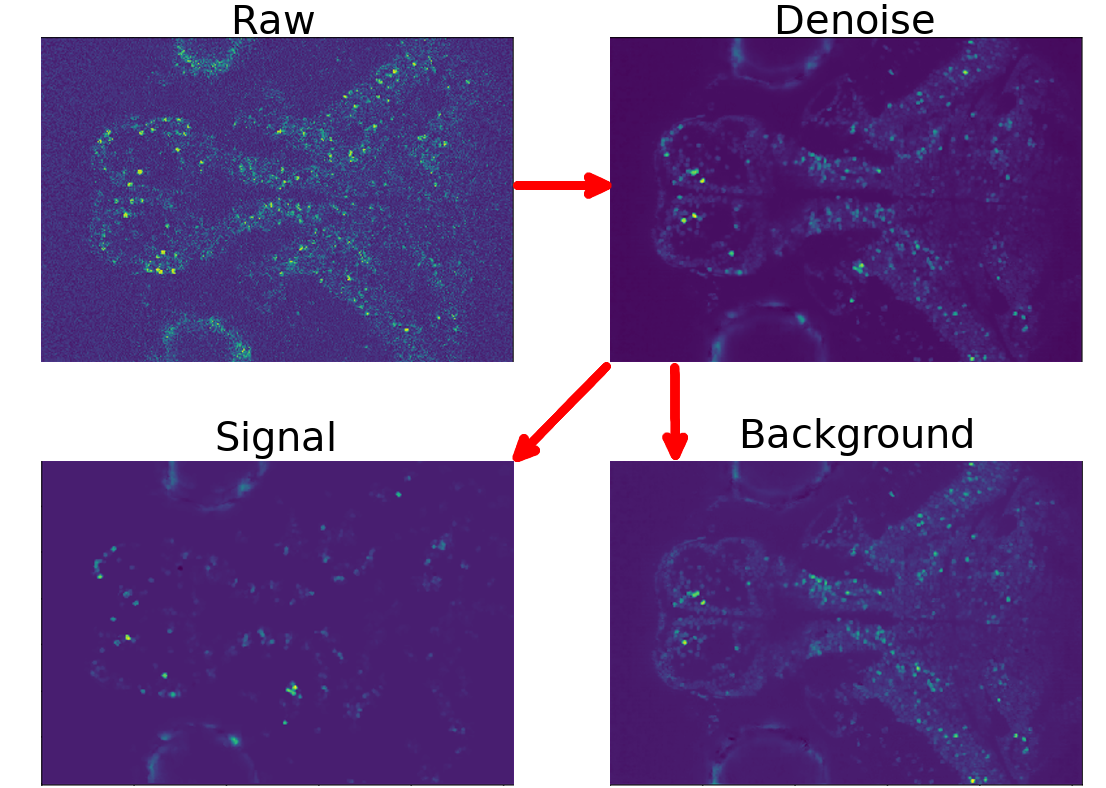
\includegraphics[width=\textwidth]{media/cnmf_arrow.png}
\end{frame}{}

\begin{frame}{Train data: LS and VP perform equally well}{$<5\%$ difference in MSE}
	\centering
	\begin{figure}
		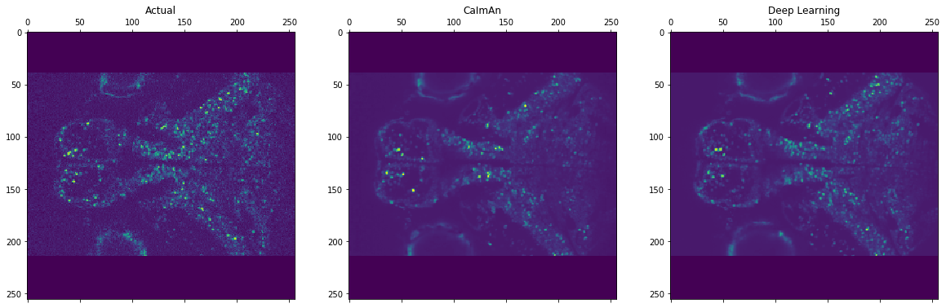
\includegraphics[width=\textwidth]{media/train_mse}
		\caption{Actual (left), least squares prediction (middle), volume prediction (right)}
	\end{figure}
\end{frame}

\begin{frame}{Test data: VP performs better}{LS has 150\% greater MSE than VP}
	\centering
	\begin{figure}
		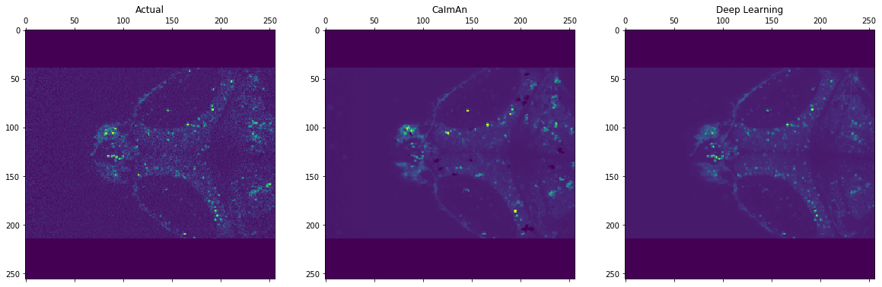
\includegraphics[width=\textwidth]{media/test_mse}
		\caption{Actual (left), least squares prediction (middle), volume prediction (right)}
	\end{figure}

\end{frame}

\begin{frame}{Masked test data: VP performs better}{LS has 40\% greater MSE than VP}
	\centering
	\begin{figure}
		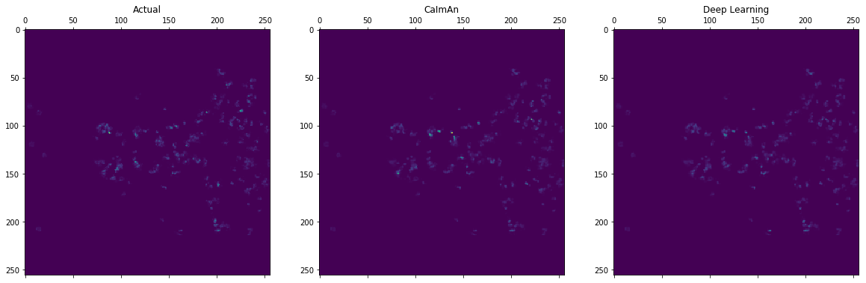
\includegraphics[width=\textwidth]{media/mask_mse}
		\caption{Actual (left), least squares prediction (middle), volume prediction (right)}
	\end{figure}
\end{frame}

\begin{frame}{ CNMF preprocessing reduces VP performance }{Evaluated loss on neuron mask}
	\begin{center}
		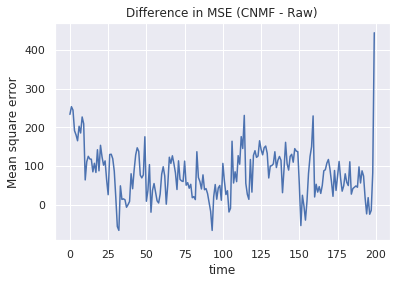
\includegraphics[height=0.7\textheight]{media/cnmf_pairwise.png}
	\end{center}
\end{frame}{}

\begin{frame}{ Extracting causal hypotheses }{Voxels used for predicted locus coeruleus activation}
% TODO
    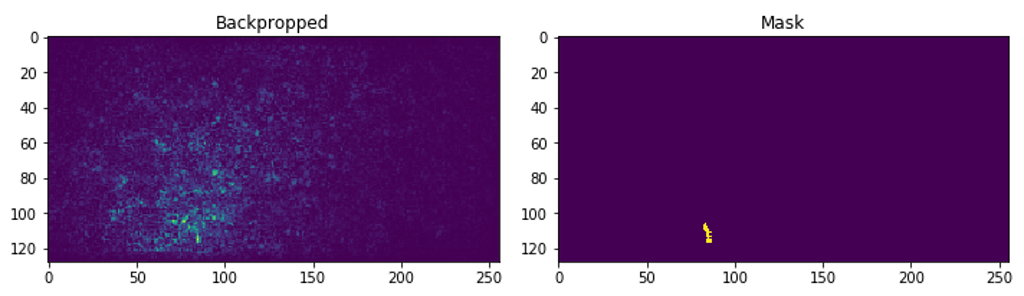
\includegraphics[width=\textwidth]{media/backprop_mask.png}
		\note{Ask model what is important; here we use backprop}
		% \note[item]{ideally show (1) variance heatmap (2) backprop very active neuron (3) backprop very quiet neuron (4) forward autodiff of a neuron (influence mapping)}
\end{frame}{}

\begin{frame}{ Voltron 549 imaging }{ Widefield @ 500Hz with Orca Flash 4.0 V2+}
    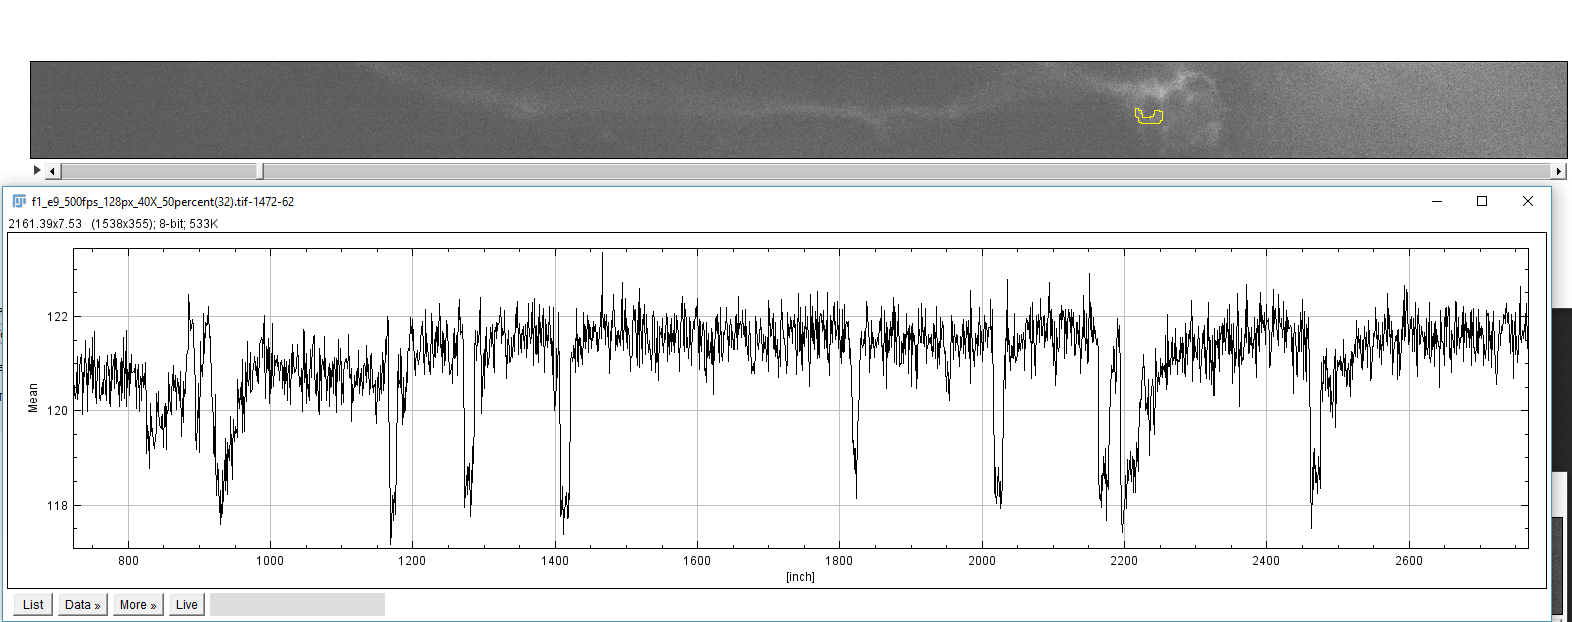
\includegraphics[width=\textwidth]{media/voltron_example_trace}
		\note{at first excited, then noticed video had major motion artifacts}
\end{frame}{}

\begin{frame}{ Voltron 549 imaging }{ Motion confounds purported APs}
	\movie[]{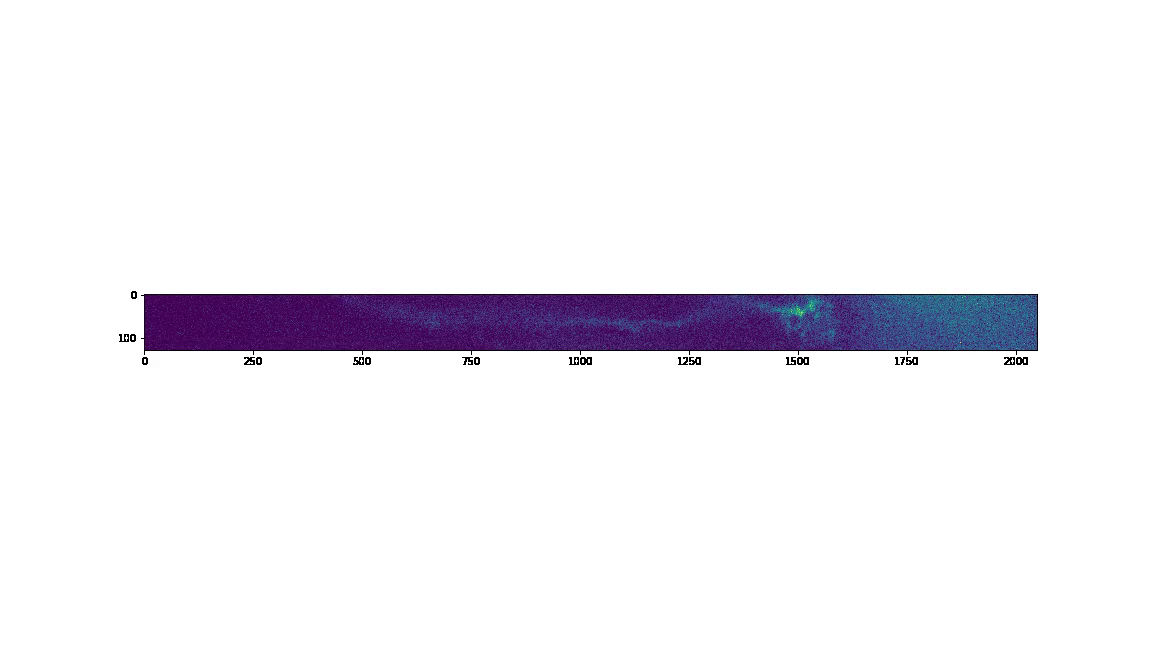
\includegraphics[width=\textwidth,center]{media/voltron_vid.png}}{media/voltron_vid.mp4}
\end{frame}{}

\begin{frame}{ Voltron pre vs post motion correction }{ After non-rigid motion correction, no APs are visible}
    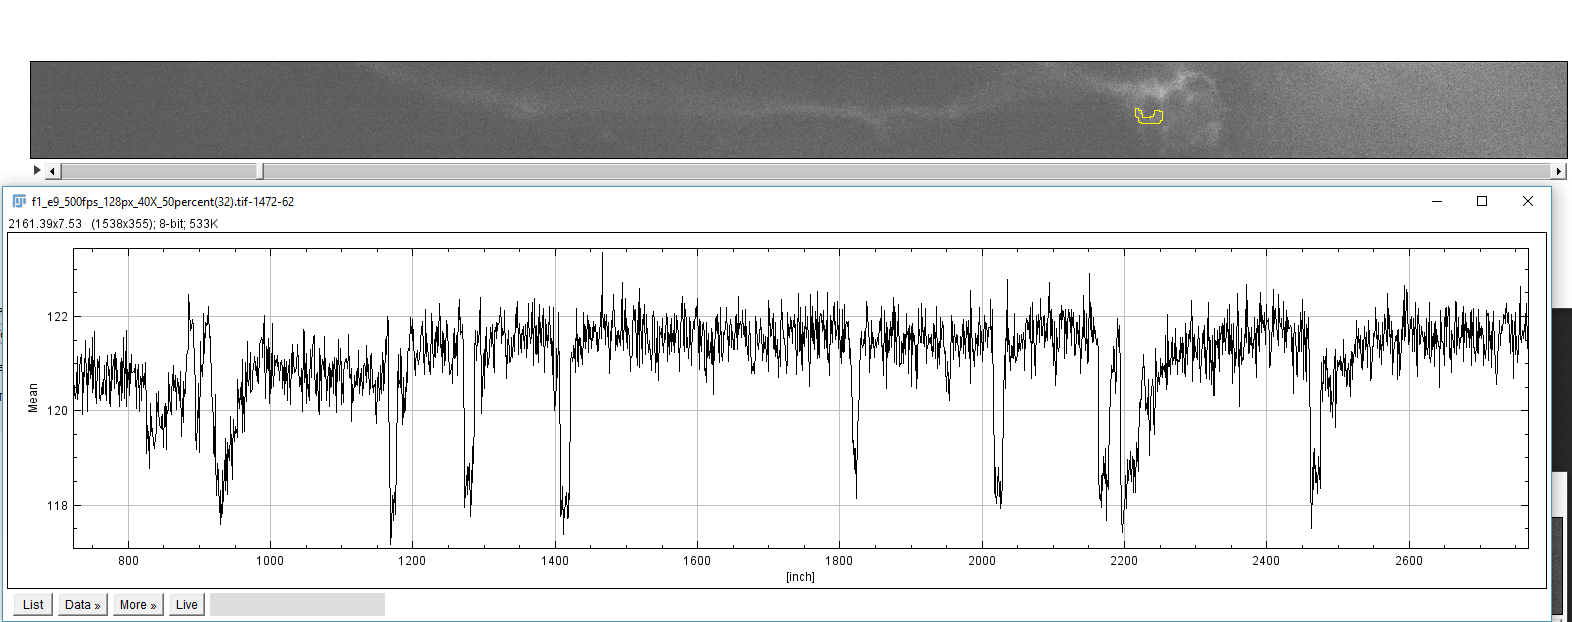
\includegraphics[width=\textwidth]{media/voltron_example_trace}
    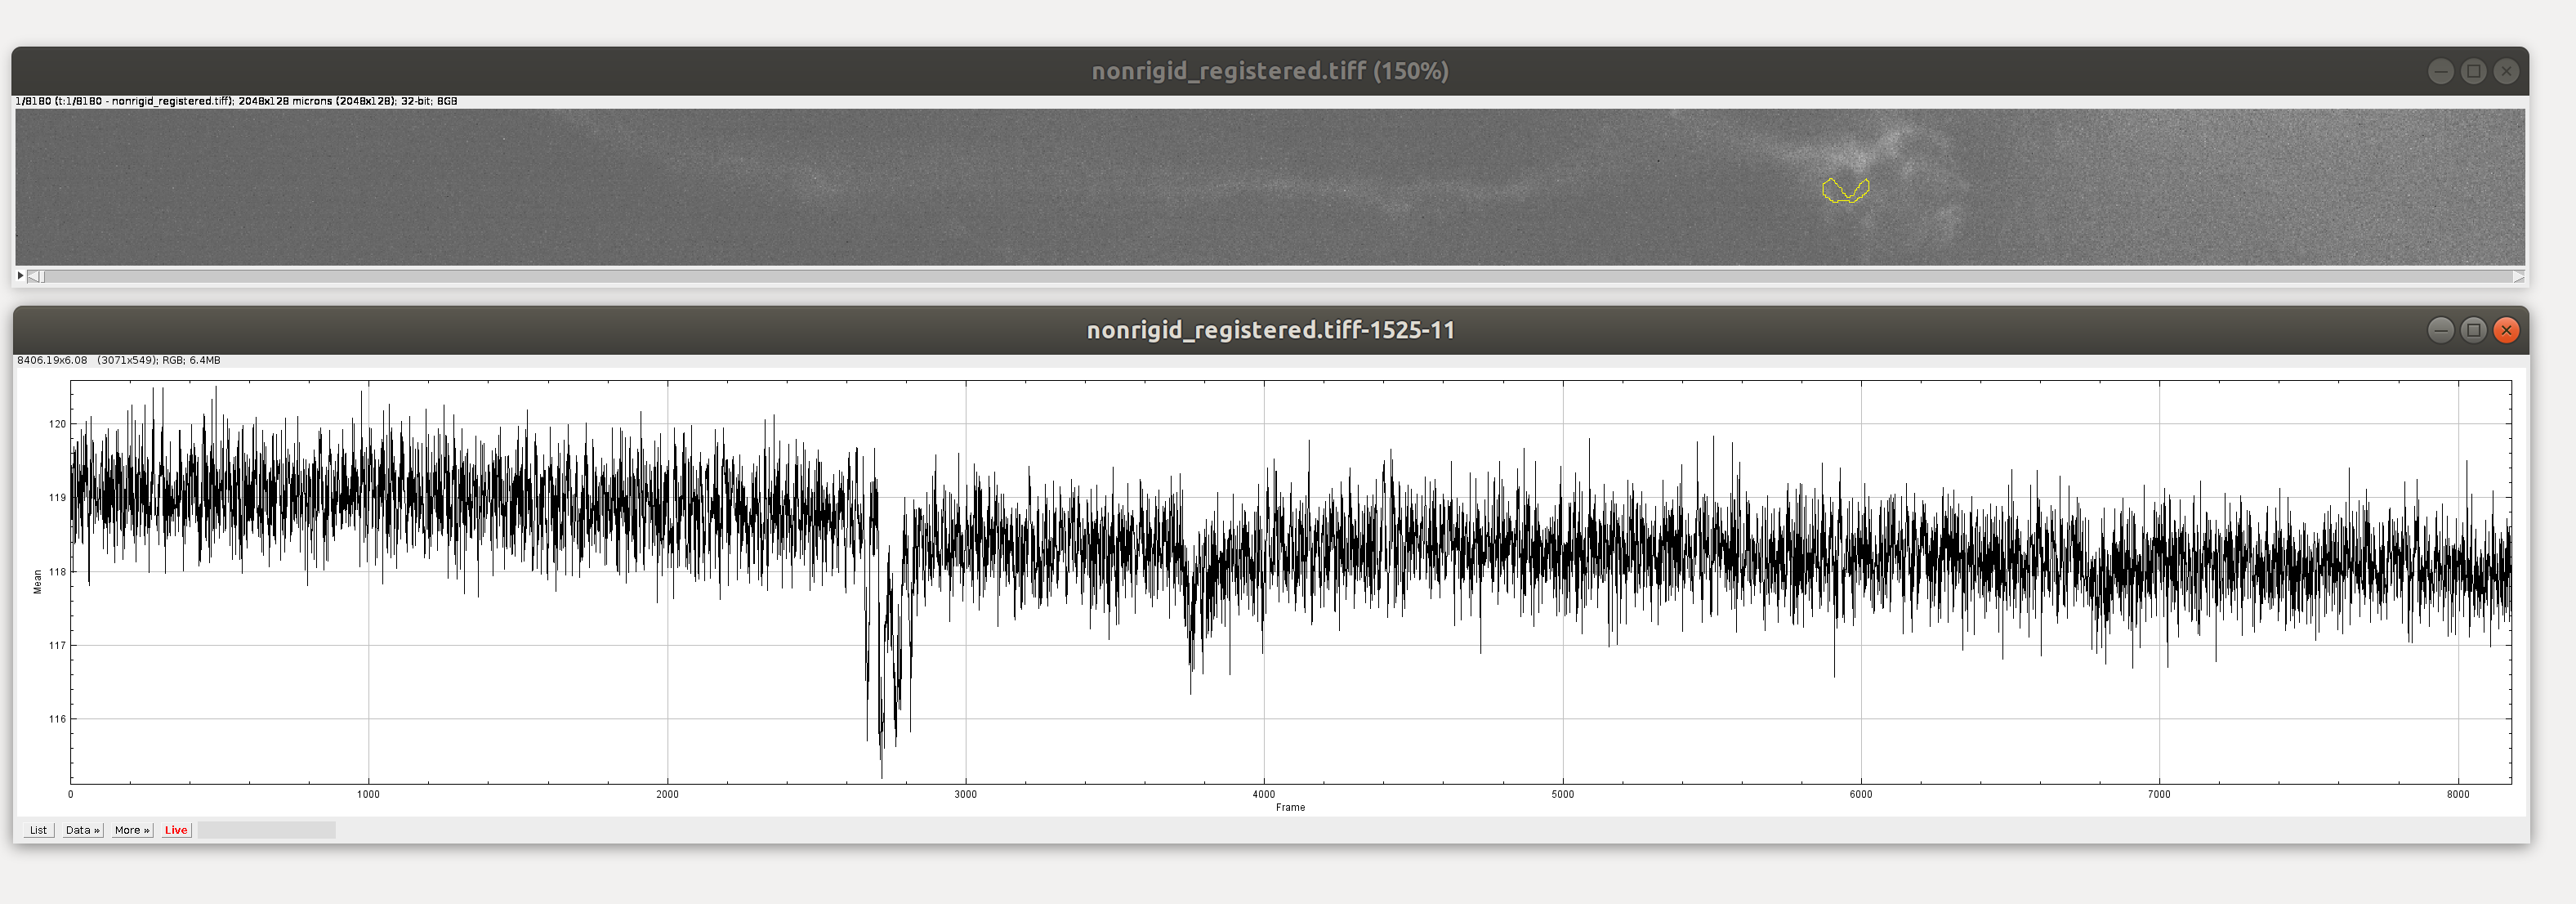
\includegraphics[width=\textwidth]{media/voltron_nonrigid}
		\note{at first excited, then noticed video had major motion artifacts}
\end{frame}{}


\begin{frame}{ Voltage dye in the near-infrared II window (1000nm-1700nm) }{ }
	\movie[]{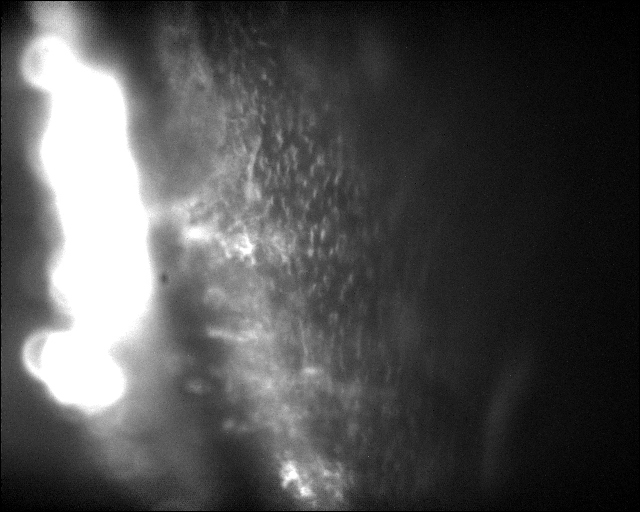
\includegraphics[height=0.45\textheight,center]{media/dai_voltage.png}}{media/dai_voltage.mp4}
	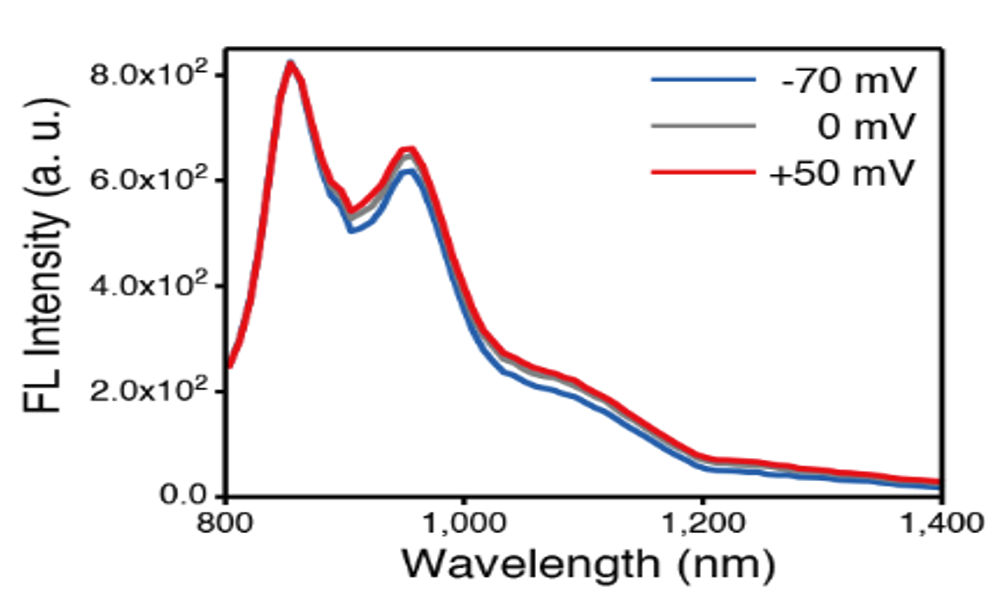
\includegraphics[height=0.4\textheight,center]{media/Spectra.png}
	\nakedfootnote{Ye Tian, Hongjie Dai \emph{unpublished}}
\end{frame}{}

\begin{frame}{ Latent space interpretation }{ }
	\begin{columns}
		\column{0.5\textwidth}
		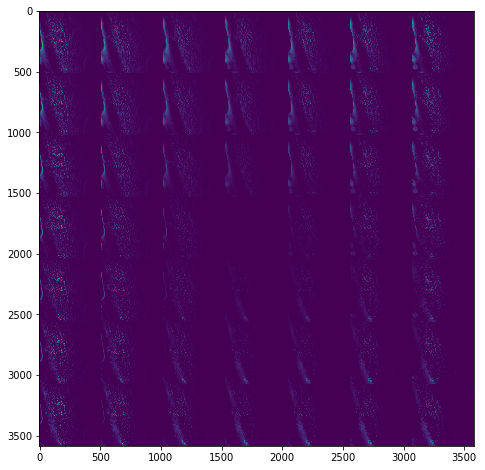
\includegraphics[width=\textwidth]{media/dai_pca.png}
		PCA
		\column{0.5\textwidth}
		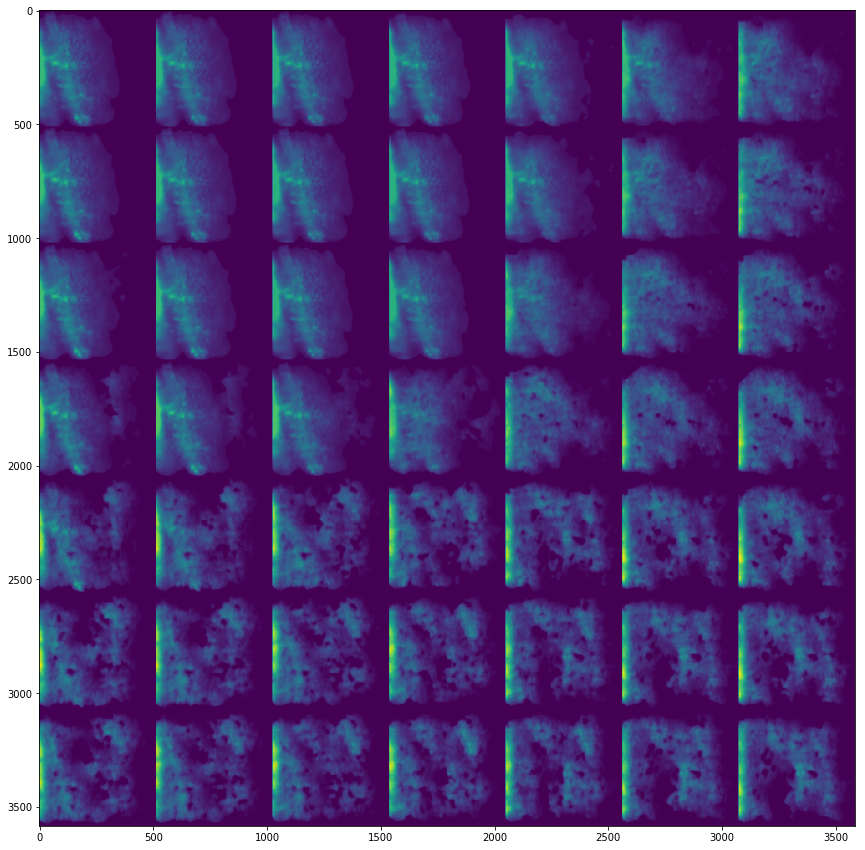
\includegraphics[width=\textwidth]{media/voltage_latent}
		Latent encoding from conv-VAE
\end{columns}
\end{frame}{}
